\documentclass[aspectratio=169]{beamer}
\usepackage{graphicx}
\usepackage{amsmath}
\usepackage{amssymb}
\usepackage[T1]{fontenc}
\usepackage[utf8]{inputenc}
\usepackage[english]{babel}

\title{EVT and Angular Distributions}
\author{Peter Trubey \\ UCSC Department of Statistics}
\date[12/18/2020]{Bruno's Lab Meeting\\12/17-18/2020}

\begin{document}

\begin{frame}
  \titlepage
\end{frame}

\begin{frame}
  \frametitle{Overview}
  \tableofcontents
\end{frame}

\section{Introduction}

\begin{frame}
  \frametitle{Introduction}
  \begin{itemize}
    \item Our goal is a framework for anomaly detection using extreme value theory
    \item Currently at least, We're still focusing on the EVT part
  \end{itemize}
\end{frame}

\begin{frame}
  \frametitle{EVT - A brief introduction}
  \begin{itemize}
    \item Why EVT?
    \item Block Maxima - GEV
    \item Thresholding - GP
  \end{itemize}
\end{frame}

\begin{frame}
  \frametitle{Block Maxima - GEV}
  \begin{itemize}
    \item GEV (Generalized Extreme Value Distribution) is a unification of three distributions:
      Frechet, Gumbel, and Weibull.
    \item For i.i.d. $x_1,\ldots,x_n$ $x_i \sim F$, $M_n = \max_{i}x_i$, if there exists some
      sequence $a_n > 0$, $b_n$ such that:
      \begin{equation*}
        \text{Pr}\left[\frac{M_n - b_n}{a_n} \leq z\right]\to G(z)
          \hspace{0.5cm}\text{as}\hspace{0.5cm}n\to\infty
      \end{equation*}
      Then $G(z)$ takes the form:
      \begin{equation*}
        G(z) = \exp\left\lbrace
            -\left[1 + \xi\left(\frac{z - \mu}{\sigma}\right)\right]^{-\xi^{-1}}
            \right\rbrace
      \end{equation*}
      Then $F$ falls into the \emph{domain of attraction} of said GEV.
  \end{itemize}
\end{frame}

\begin{frame}
  \frametitle{Thresholding - GP}
  \begin{itemize}
    \item We look now at the distribution of excesses $y$ over a threshold $u$.
      \begin{equation*}
        \text{Pr}[X > u + y \mid X > u] = \frac{1 - F(u + y)}{1 - F(u)}, \hspace{1cm}y > 0
      \end{equation*}
      If $F$ is in the domain of attraction of a GEV, then $\text{Pr}[X > u + y \mid X > u]$ converges to
      \begin{equation*}
        H(y) = 1 - \left(1 + \frac{\xi y}{\sigma}\right)^{-\xi^{-1}},
      \end{equation*}
      the Generalized Pareto distribution.
      \item We set a high threshold by some criteria, then model excesses over that threshold using GP.
  \end{itemize}
\end{frame}

\begin{frame}
  \frametitle{Multivariate EVT}
  \begin{itemize}
    \item Useful to standardize each $X_i$ according to its marginal distribution
    \item Standardization occcurs as:
      \begin{equation}
        z_j = \left(1 + \xi\frac{x_j - b_{t,j}}{a_{t,j}}\right)_{+}^{1/\xi}
      \end{equation}
			where $b_{t,j} = \hat{F}^{-1}(1 - 1/t)$. 
    \item Note that $Z_j > 1\implies X_j > b_{t,j}$
    \item $\max_j Z_j \sim \text{Pareto}$
		\item $a$, $\xi$ are currently found by MLE.  Not ideal, I know.
  \end{itemize}
\end{frame}

\begin{frame}
  \frametitle{Multivariate EVT}
  \begin{itemize}
    \item Assume the existence of a limit measure $\mu$ on ${\bf Z}$ such that:
    \begin{equation*}
      n\text{Pr}\left(\frac{V_1}{n} \geq v_1 \text{ or }\ldots\text{ or }\frac{V_d}{n}\geq v_d\right)
      \rightarrow \mu\left([{\bf 0}, {\bf v}]^C\right)
    \end{equation*}
    \item $\mu$ is the asymptotic distribution of ${\bf Z}$ in extreme regions.
    \item $\mu$ features the homogeneity property, $\mu(t\cdot) = t^{-1}\mu(\cdot)$.
  \end{itemize}
\end{frame}

\begin{frame}
  \frametitle{Pseudo-Polar Representation}
  Given the homogeneity property, we can decompose ${\bf Z}$ into two components, radial and angular:
    \begin{equation*}
      \begin{aligned}
        R({\bf Z}) &= \lVert {\bf Z}\rVert_{\infty} = \max_i v_i\\
        {\bf V} &= \frac{{\bf Z}}{R} \in S_{\infty}^{d-1}
      \end{aligned}
    \end{equation*}
  where $S_{\infty}^{d-1}$ is the positive orthant of the unit hypercube in $R^d$.
\end{frame}

\begin{frame}
  \frametitle{Spectral Measure}
  For $B \subset S_{\infty}^{d-1}$, define the \emph{Spectral Measure}:
  \begin{equation*}
    \Omega(B) = \mu[{\bf z}: R({\bf z}) > 1, {\bf V} \in B].
  \end{equation*}
  Then,
  \begin{equation*}
    \mu[{\bf z}:R(z)>t, {\bf V}\in B] = t^{-1}\Omega(B).
  \end{equation*}
  Thus $t$ is independent of $\Omega$, the spectral measure.  This is completed as a
    probability measure as:
  \begin{equation*}
    \text{Pr}\left({\bf V} \in B \mid r > 1\right) = \frac{\Omega(B)}{\Omega(S_{\infty}^{d-1})}.
  \end{equation*}
  So conditional on at least one dimension exceeding its threshold, we can hold the
  angular measure independent of the magnitude.
\end{frame}

\section{Methodology \& Results}

\subsection{Polar Coordinate Transformation}

\begin{frame}
  \frametitle{Polar Coordinate Transformation}
  \begin{itemize}
    \item One way
      \begin{equation*}
        \begin{aligned}
          y_1     &= r\cos\theta_1,\\
          y_2     &= r\sin\theta_1\cos\theta_2\\
                  &\vdots\\
          y_{d-1} &= r\sin\theta_1\ldots\sin\theta_{d-2}\\
          y_{d}   &= r\sin\theta_1\ldots\sin\theta_{d-1}
        \end{aligned}
      \end{equation*}
    \item The other way
      \begin{equation*}
        \begin{aligned}
          \theta_1     &= \cos^{-1}\left[\frac{y_1}{\lVert y_{1:d}\rVert_2}\right]\\
          \theta_2     &= \cos^{-1}\left[\frac{y_2}{\lVert y_{2:d}\rVert_2}\right]\\
                       &\vdots\\
          \theta_{d-1} &= \cos^{-1}\left[\frac{y_{d-1}}{\lVert y_{(d-1):d}\rVert_2}\right].
        \end{aligned}
      \end{equation*}
  \end{itemize}
\end{frame}

\begin{frame}
  \frametitle{Polar Coordinate Transformation Effects}
  \begin{figure}
    \centering
    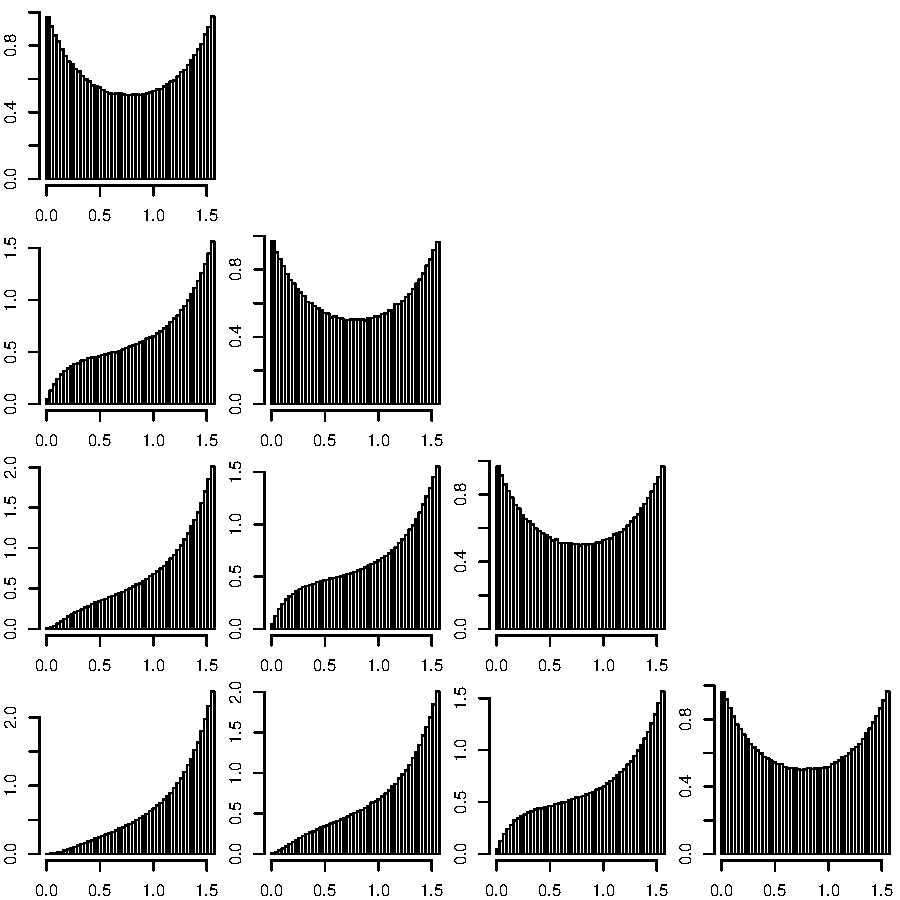
\includegraphics[scale = 0.5]{./images/independent_transformed}
	\end{figure}
\end{frame}

\subsection{Projected Gamma Distribution}

\begin{frame}
  \frametitle{Projected Gamma Distribution}
  Consider $d$ independent Gammas
  \begin{equation}
      f({\bf y}\mid{\bf \alpha},{\bf \beta}) = \prod_{j = 1}^d\text{Ga}(y_j\mid\alpha_j,\beta_j),
  \end{equation}
  Use polar coordinate transformation, then integrate out $r$.
  \begin{equation}
      \text{PG}({\bf \theta}\mid{\bf \alpha},{\bf \beta}) = \frac{\Gamma(A)\beta_d^{\alpha_d}}{B^A
      \Gamma(a_d}\left(\prod_{j = 1}^{d-1}\frac{\beta_j^{\alpha_j}}{\Gamma(\alpha_j)}(\cos\theta_j
      )^{\alpha_j - 1}(\sin\theta_j)^{(\sum_{h = j + 1}^d\alpha_h) - 1}\right)\mathcal{I}_{(0,\pi/2
      )^{d-1}}({\bf \theta})
  \end{equation}
  where
  \begin{equation}
      A = \sum_{j = 1}^d\alpha_j \hspace{1cm}\text{and}\hspace{1cm}
      B = \beta_1\cos\theta_1 + \sum_{j = 2}^{d-1}\left(\beta_j\cos\theta_j\prod_{
          i = 1}^{j-1}\sin\theta_i\right) + \beta_d\prod_{j = 1}^d-1\sin\theta_j.
  \end{equation}
\end{frame}

\begin{frame}
  \frametitle{Projected Gamma, Cont.}
  \begin{itemize}
    \item Let ${\bf y}^{\prime} = \frac{{\bf y}}{r}$, ${\bf y} = r{\bf y}^{\prime}$.
    \item Gibbs sampling updates to $\alpha$, $\beta$ possible with latent $r$.
      \begin{equation*}
        r_i\mid {\bf \alpha}, {\bf \beta} \sim \text{Ga}\left(r_i\mid  \sum_j\alpha_j, \sum_j \beta_jy_{ij}^{\prime}  \right)
      \end{equation*}
    \item For Projected Gamma, information between dimensions is effectively communicated through the latent $r$.
  \end{itemize}
\end{frame}

\begin{frame}
  \frametitle{Projected Gamma, Cont.}
	\begin{figure}
		\centering
    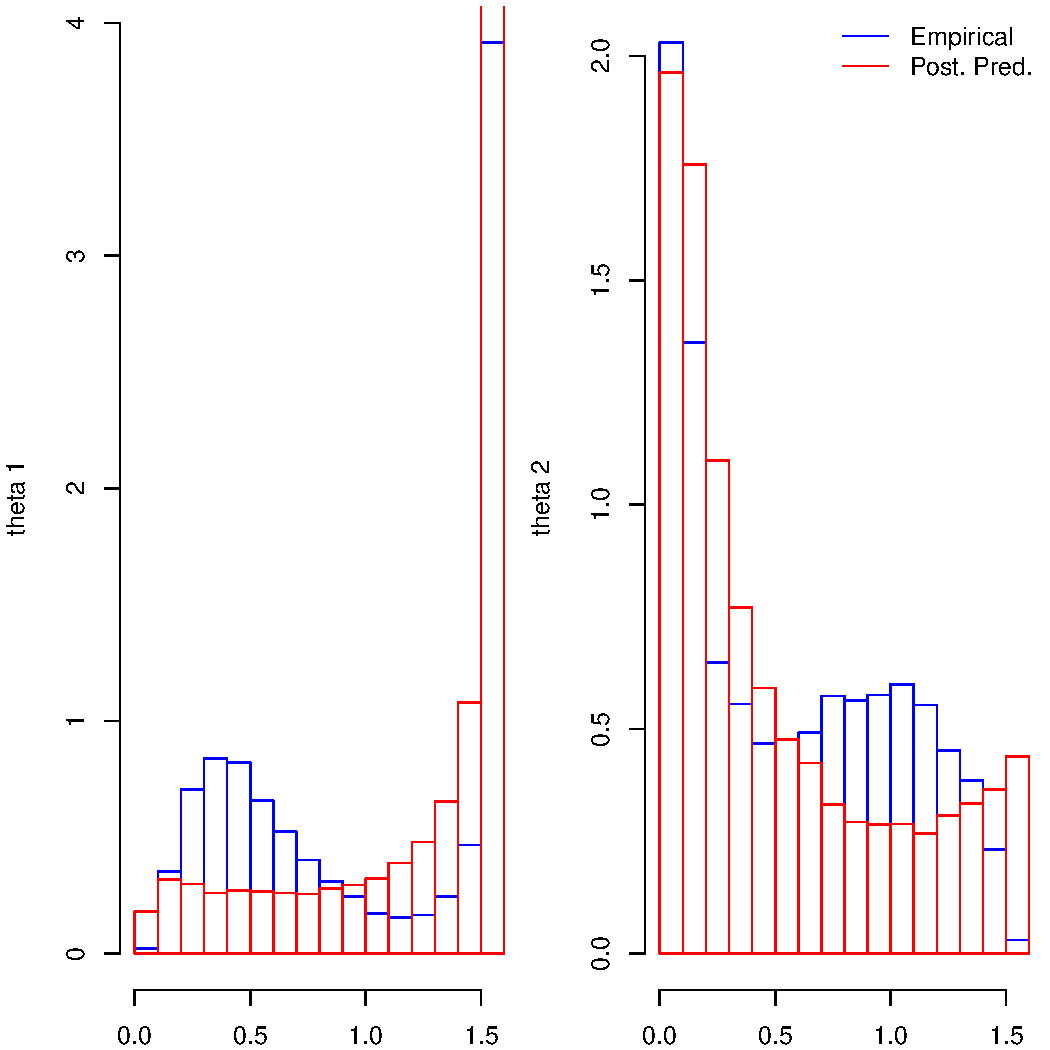
\includegraphics[scale = 0.4]{./images/justification_for_more_complex_models}
	\end{figure}
\end{frame}

\subsection{Finite Mixture of Projected Gammas}

\begin{frame}
  \frametitle{Finite Mixture of Projected Gammas}
  \begin{equation*}
    \begin{aligned}
      \text{MPG}({\bf \theta}\mid {\bf \lambda}, {\bf \alpha}, {\bf \beta}) &= \sum_{j = 1}^J\lambda_i\text{PG}(\alpha_i,\beta_i) \nonumber \\
      &= \int \text{MPG}({\bf \theta}, {\bf \gamma} \mid{\bf \alpha},{\bf \beta})d\gamma \nonumber \\
      &= \int \prod_{j = 1}^J\left[\lambda_j\text{PG}({\bf \theta}\mid\alpha_j,\beta_j)\right]^{\gamma_j}\text{d}\gamma \\
      &= \int_{\gamma}\int_{r}\lambda_j^{\gamma_j}\prod_{k = 1}^K\text{Ga}(r{\bf y}^{\prime}\mid{\bf \alpha_j},{\bf \beta_j})^{\gamma_j}\lvert\text{Jac}\rvert \text{d}r\text{d}\gamma
    \end{aligned}
  \end{equation*}
\end{frame}

\begin{frame}
  \frametitle{Finite Mixture of Projected Gammas - cont.}
  \begin{figure}[h!]
    \centering
    %\caption{Posterior Predictive distribution from Mixture of Projected Gammas model with
    %         15 mixture components, built on declustered IVT data.}
    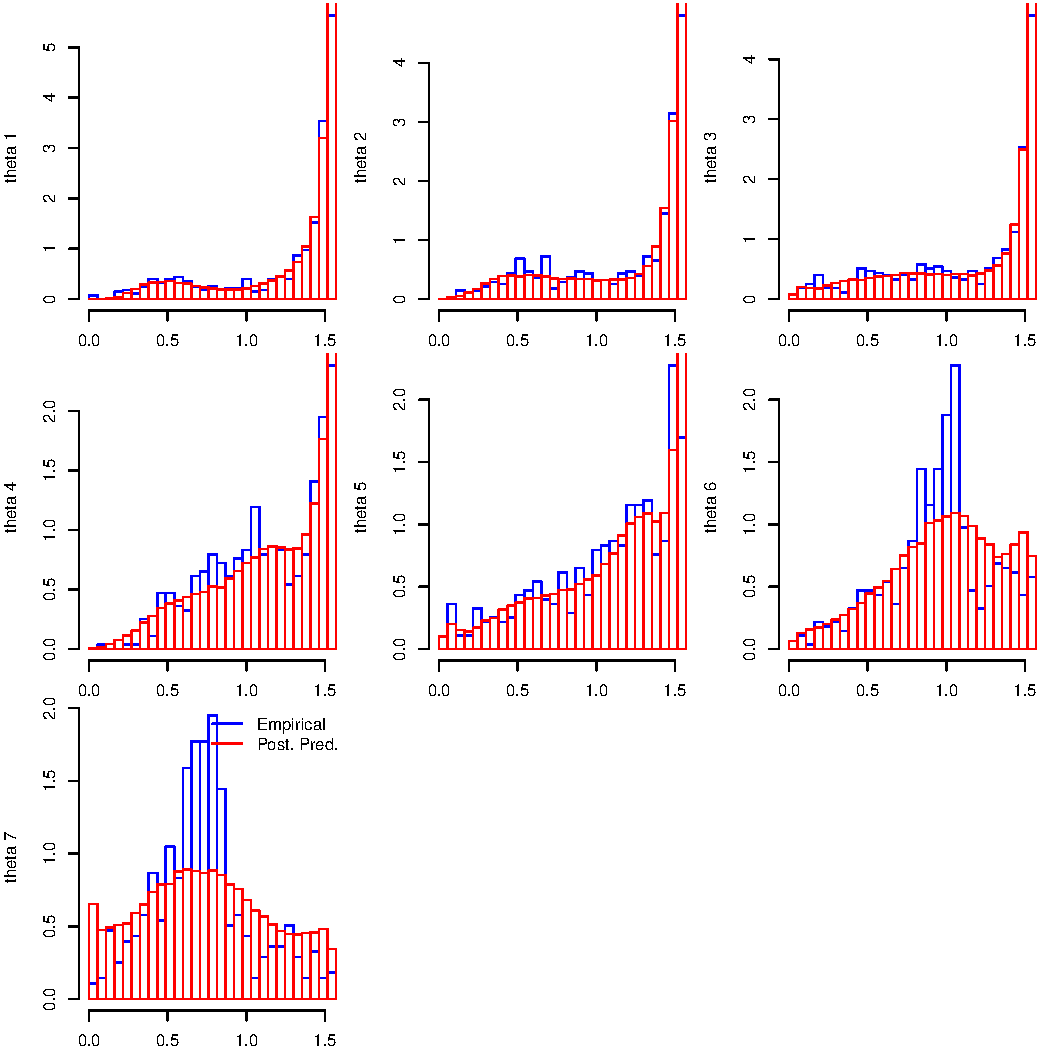
\includegraphics[scale = 0.43]{./images/mpg_15_emp_v_pred_decluster}
  \end{figure}
\end{frame}

\subsection{DP Mixture of Projected Gammas, Independent Prior}

\begin{frame}
  \frametitle{DP Mixture of Projected Gammas, Independent Gamma Prior}
  \begin{equation*}
    \begin{aligned}
      \theta_i &\sim \text{PG}\left(\theta_i\mid ({\bf \alpha}_i, {\bf \beta}_i) \right)\\
      ({\bf \alpha}_i, {\bf \beta}_i) &\sim G_i\\
      G_i &\sim \text{DP}\left(\eta, G_0\left(({\bf \alpha}_i, {\bf \beta}_i)\mid ({\bf a}_{\alpha}, {\bf b}_{\alpha}, {\bf a}_{\beta}, {\bf b}_{\beta}) \right)\right)\\
       ({\bf a}_{\alpha}, {\bf b}_{\alpha}, {\bf a}_{\beta}, {\bf b}_{\beta}) &\sim P\left(({\bf a}_{\alpha}, {\bf b}_{\alpha}, {\bf a}_{\beta}, {\bf b}_{\beta})\right)\\
       \eta &\sim \text{Ga}(a_{\eta},b_{\eta})
    \end{aligned}
  \end{equation*}
  with
  \begin{equation*}
      \begin{aligned}
      G_0\left(({\bf \alpha}_i, {\bf \beta}_i)\right) &= \text{Ga}(\alpha_1\mid a_{\alpha_1},b_{\alpha_1})\prod_{j = 2}^d\text{Ga}(\alpha_j\mid a_{\alpha_j}, b_{\alpha_j})\text{Ga}(\beta_j\mid a_{\beta_j}, b_{\beta_j})\\
      P(({\bf a}_{\alpha}, {\bf b}_{\alpha}, {\bf a}_{\beta}, {\bf b}_{\beta})) &= \text{Ga}(a_{\alpha_1})\text{Ga}(b_{\alpha_1})\prod_{j = 2}^d\text{Ga}(a_{\alpha_j})\text{Ga}(b_{\alpha_j})\text{Ga}(a_{\beta_j})\text{Ga}(b_{\beta_j})
      \end{aligned}
  \end{equation*}
\end{frame}

\begin{frame}
  \frametitle{DP Mixture of Projected Gammas, Independent Gamma Prior - Cont.}
  \begin{figure}
    \centering
    %\caption{Dirichlet Process Mixture Model with Projected Gamma kernel, independent Gamma priors
    %        using declustered IVT data.}
    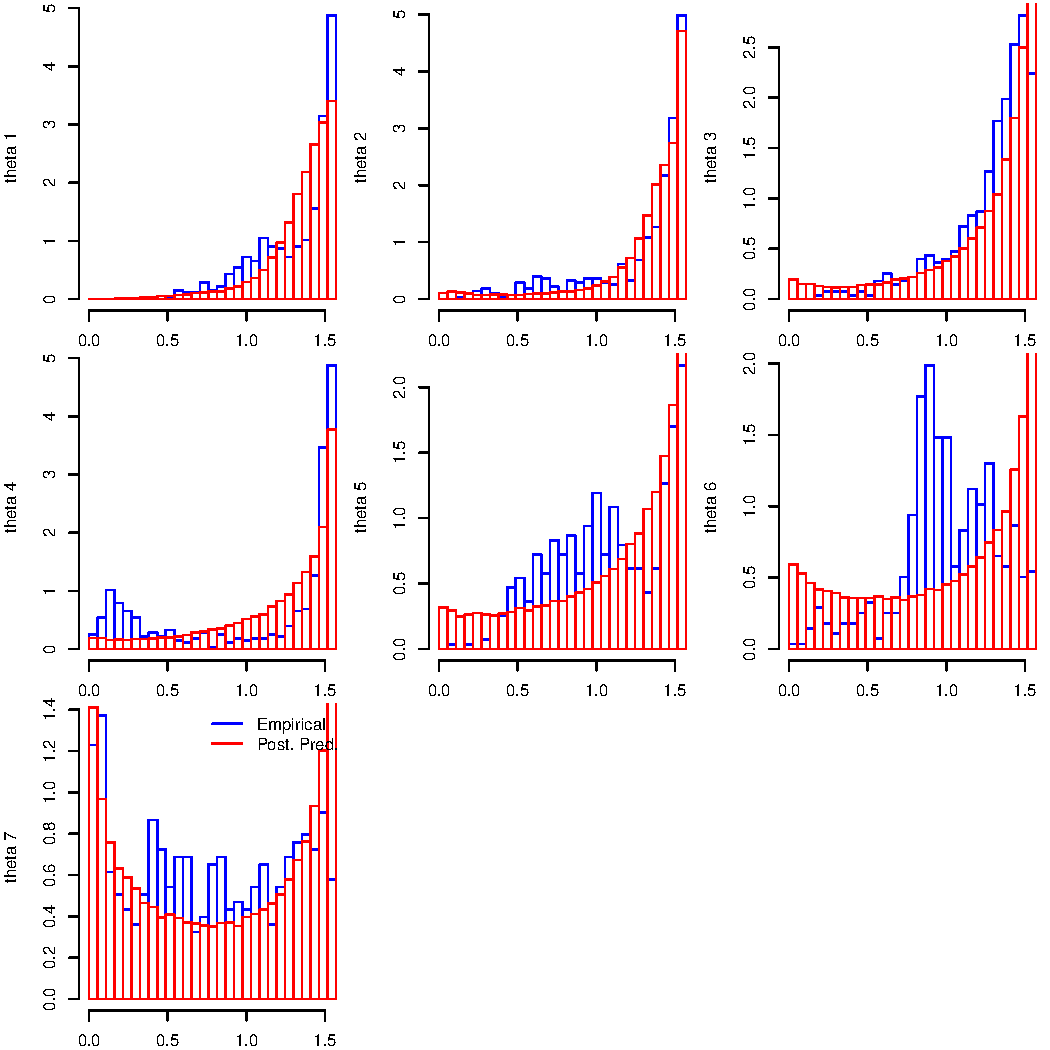
\includegraphics[scale = 0.43]{./images/dpmpg_emp_v_pred_decluster}
  \end{figure}
\end{frame}

\subsection{DP Mixture of Multivariate Normals}

\begin{frame}
  \frametitle{DP Mixture of Multivariate Normals on Probit Space}
  \begin{itemize}
    \item $\theta \in [0,\pi/2]$
      \begin{itemize}
        \item Jitter and rescale to $\theta^{\prime} \in [\epsilon, 1 - \epsilon]$
        \item Then $W = \Phi^{-1}(\theta^{\prime})$
      \end{itemize}
    \item Then develop a hierarchical multivariate normal, with length of response $d-1$.
  \end{itemize}
  \begin{equation*}
    \begin{aligned}
      W_i &\sim \mathcal{N}_d\left(\mu_i, \Sigma_i\right)\\
      \mu_i, \sigma_i &\sim G_i\\
      G_i &\sim \text{DP}(\eta, G_0(\mu_i,\Sigma_i\mid\mu_0,\Sigma_0))\\
      &\hspace{1cm}G_0(\mu_i,\Sigma_i\mid\mu_0,\Sigma_0) &=
          \mathcal{N}_d(\mu_i\mid\mu_0,\Sigma_0)\text{IW}(\Sigma\mid\nu,\psi)\\
      \mu_0 &\sim \mathcal{N}_d\left({\bf u},{\bf S}\right)\\
      \Sigma_0 &\sim \text{IW}(\nu_0,\psi_0)\\
      \eta &\sim \text{Ga}(\alpha, \beta)
    \end{aligned}
  \end{equation*}
\end{frame}

\begin{frame}
  \frametitle{DP Mixture of Multivariate Normals on Probit Space - cont.}
  \begin{figure}
    \centering
    %\caption{Dirichlet Process mixtue model with multivariate normal kernel over probit space cast
    %          on angular representation using declustered IVT dataset}
    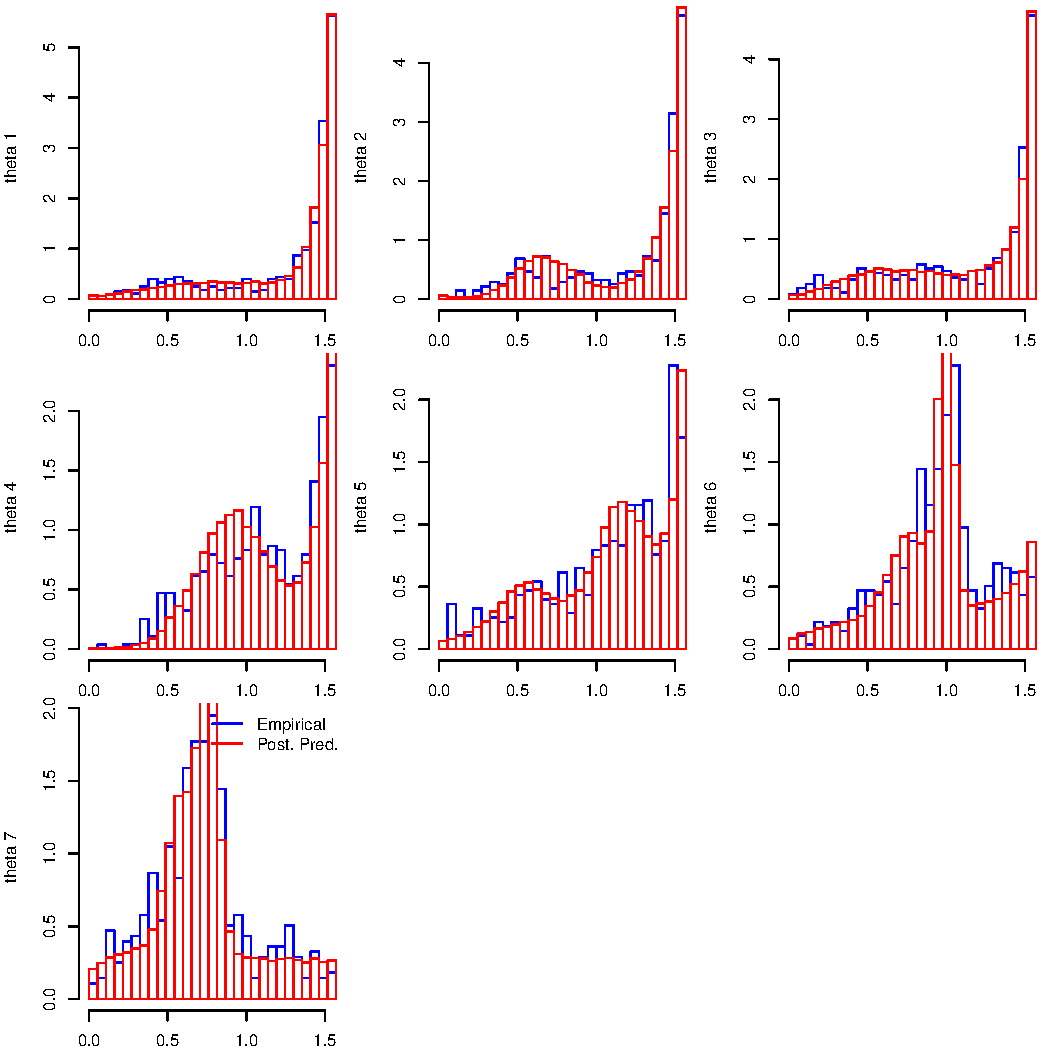
\includegraphics[scale = 0.43]{./images/dpmp2_emp_v_pred_decluster}
  \end{figure}
\end{frame}

\subsection{DP Mixture of Projected Gammas, LogNormal Prior}

\begin{frame}
  \frametitle{DP Mixture of Projected Gammas, LogNormal Prior}
  \begin{itemize}
    \item The Normal Normal model operated in $d-1$-dimensional space without considering the transformation
      that brought it there.
    \item If we want to operate in $d$-dimensional space with $d-1$ degrees of freedom, then Projected Gamma
      is a good base distribution.
    \item Placing a multivariate log-normal prior on $\alpha$, we can \emph{potentially} communicate information
      across dimensions more effectively than with $r$ alone.
  \end{itemize}
  \begin{equation*}
    \begin{aligned}
      \theta_i &\sim \text{PG}(\theta_i\mid \alpha_i,\beta_i)\\
      r_i &\sim \text{Ga}(r_i\mid \alpha_i,\beta_i)\\
      (\alpha_i,\beta_i) &\sim \text{DP}\left((\alpha_i,\beta_i)\mid \eta, G_0\right)\\
      G_0 &= \text{Log}\mathcal{N}(\alpha_i\mid\mu,\Sigma)\prod_{j = 2}^d\text{Ga}(\beta_{ij}\mid a, b)\\
      \mu &\sim \mathcal{N}(\mu\mid\mu_0,\Sigma_0)\\
      \Sigma &\sim \text{IG}(\Sigma\mid\nu,\psi)
    \end{aligned}
  \end{equation*}
\end{frame}


\begin{frame}
  \frametitle{DP Mixture of Projected Gammas, LogNormal Prior - cont.}
  \begin{figure}
    \centering
    %\caption{DP-MPG with Lognormal Prior on $\alpha$, fitted to IVT data.}
    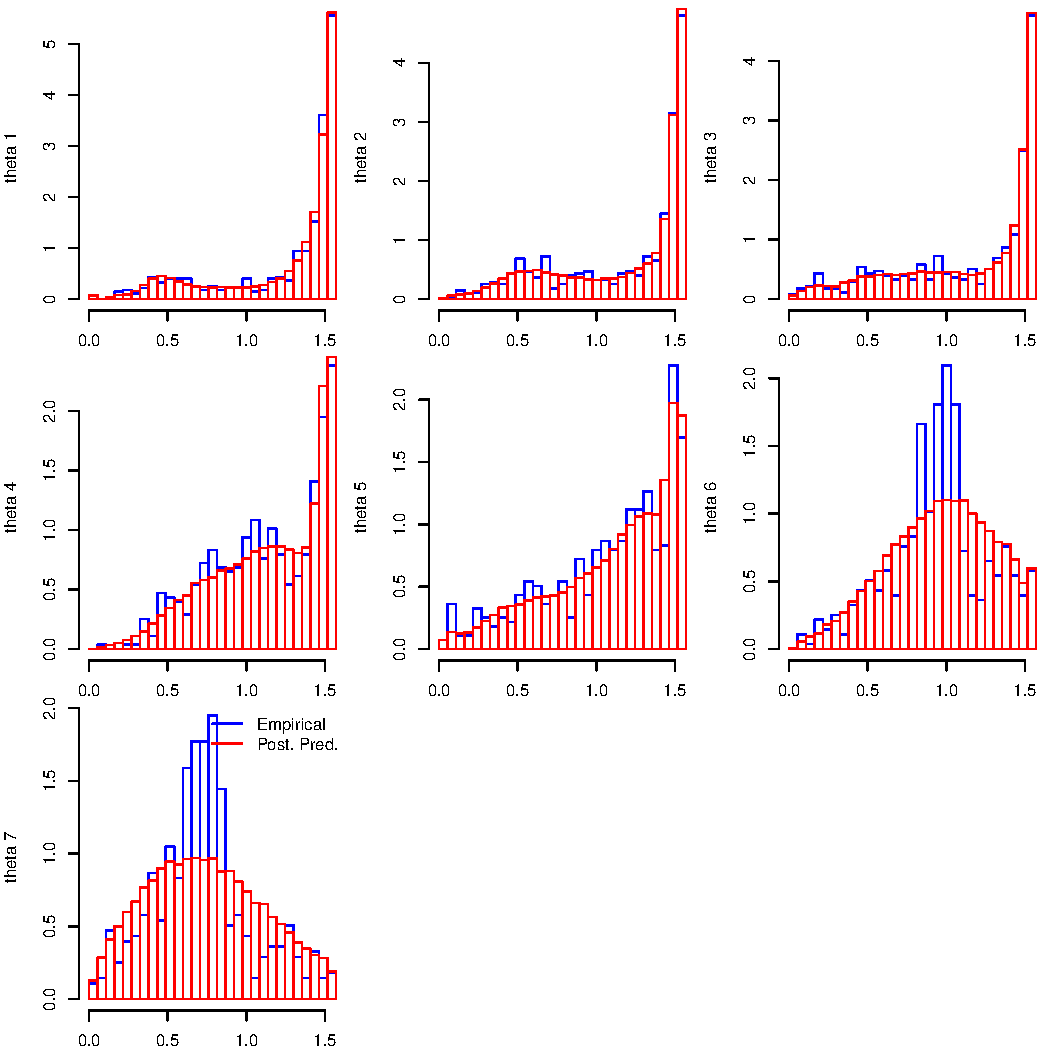
\includegraphics[scale = 0.43]{./images/dppgln_emp_v_pred_2_1e1}
  \end{figure}
\end{frame}

\begin{frame}
	\begin{center}
		{\huge \emph{fin}}
	\end{center}
\end{frame}



\end{document}
